\documentclass{beamer}
\usetheme{metropolis}

\usepackage[utf8]{inputenc}
\usepackage[T1]{fontenc}
\usepackage[french]{babel}
\usepackage{listings}
\usepackage{graphicx}
\usepackage{hyperref}
\usepackage{xcolor}
\usepackage{svg}
% Define custom colors
\definecolor{commentgray}{rgb}{0.5, 0.5, 0.5}
\definecolor{keywordorange}{rgb}{0.8, 0.4, 0.0}
\definecolor{typeblue}{rgb}{0.2, 0.6, 1.0}
\definecolor{fggray}{rgb}{0.4, 0.4, 0.4}

\lstset{
    language=nix,
    basicstyle=\ttfamily\color{fggray},
    keywordstyle=\color{keywordorange}\bfseries,
    stringstyle=\color{green!60!black},
    commentstyle=\color{commentgray},
    morekeywords={with, let, in, rec, import, derivation},
    numbers=none,
    showstringspaces=false,
}

\title{Nix : Révolutionner la gestion de paquets}
\author{Emeric Laberge}
\date{\today}

\begin{document}

\maketitle

\begin{frame}{Plan de la présentation}
	\tableofcontents
\end{frame}

\section{Introduction}

\begin{frame}{Qu'est-ce qu'un gestionnaire de paquets ?}
  \begin{itemize}
    \item Outil de gestion des dépendances logicielles
    \item Permet d'installer, mettre à jour et désinstaller des paquets
  \end{itemize} 
\end{frame}

    \begin{frame}{En quoi c'est utile ?}
    \begin{itemize}
      \item On peut installer des logiciels sans avoir à les compiler 
      \item Facilite la gestion des dépendances (un programme peut en dépendre
        de plusieurs)
      \item Permet de garder les logiciels à jour
    \end{itemize}
  \end{frame}

\begin{frame}{Problèmes actuels}
  \begin{itemize}
    \item Conflits de dépendances, notamment entre plusieurs versions d'une même
      dépendance, 
    \item Environnements non reproductibles, un programme peut fonctionner sur
      une machine mais pas sur une autre. 
    \item On doit utiliser des outils supplémentaires pour gérer ces problèmes
      (virtualenv, conda, docker, etc.)
  \end{itemize}
\end{frame}

\begin{frame}{La solution?}
  \begin{center}
    \Huge{\textbf{Nix}}
  \end{center}
  \begin{figure}
    \centering
    
\includegraphics[width=0.3\linewidth]{nix-logo.pdf}
  \end{figure}
\end{frame}


  \begin{frame}{Qu'est-ce que Nix?}
    \begin{itemize}
      \item \textbf{Quoi} : Gestionnaire de paquets purement fonctionnel avec 
        plus de \textbf{100 000} paquets \footnotemark[1]
      \item \textbf{Où} : Disponible sur Linux, MacOS et 
        autres \textit{Unix-like}
        \item \textbf{Auteur} : Eelco Dolstra
        \item \textbf{Date de sortie} : 15 juin 2003
        \item \textbf{Contexte} : Développé dans le cadre de sa thèse de
          doctorat \textit{The Purely Functional Software Deployment
          Model} (2006) \footnotemark[2]
        \item \textbf{Autres détails} : Langage de programmation à part entière,
          logiciel libre (GNU LGPLv2.1)
      \end{itemize}
    \footnotetext[1]{\href{https://nixos.org/}{Site officiel de Nix}}
    \footnotetext[2]{\href{https//edolstra.github.io/pubs/phd-thesis.pdf}{The
    Purely Functional Software Deployment Model}}
\end{frame}

\begin{frame}{Avantages de Nix}
  \textbf{\underline{Reproductibilité}} :
  \begin{itemize}
    \item Paquets sont \textit{build} de manière isolée les uns des autres.
  \end{itemize}
  \textbf{\underline{Déclaratif}} :
  \begin{itemize}
    \item Facile de partager des n'importe quel type d'environnement
      production pour des projets et ce \textbf{peu importe la machine et les
      langages de programmation utilisés}
    \item Les dépendances sont déclarées dans un fichier \textit{.nix}
  \end{itemize}
  \textbf{\underline{Fiabilité}} :
  \begin{itemize}
    \item L'ajout ou la mise à jour d'un paquet \textbf{ne peut pas} affecter
      les autres paquets. 
    \item Possibilité de \textbf{rollback} en cas de problème.
  \end{itemize}
\end{frame}

\section{Comment l'installer?} 

\begin{frame}{Installation}
  \textbf{Sur Linux} :
  \begin{center}
    \vspace{-0.3cm}
    \texttt{curl -L https://nixos.org/nix/install | sh}
    \vspace{-0.3cm}
  \end{center}
  \rule{\linewidth}{0.6pt}
  \textbf{Sur MacOS} :
  \begin{center}
    \vspace{-0.3cm}
    \texttt{sh <(curl -L https://nixos.org/nix/install)} 
    \vspace{-0.3cm}
  \end{center} 
  \rule{\linewidth}{0.6pt}
  \textbf{Sur Windows (WSL2)} : 
  \begin{center}
    \vspace{-0.3cm}
    \texttt{sh <(curl -L https://nixos.org/nix/install) --daemon} 
    \vspace{-0.3cm}
  \end{center}
\end{frame}

\section{Fonctionnement Technique}

\begin{frame}[fragile]{Aperçu de la syntaxe Nix}
    \begin{itemize}
        \item \textbf{Valeurs de base :}
            \begin{itemize}
                \item Chaînes : \lstinline|"hello world"|
                \item Booléens : \lstinline|true|, \lstinline|false|
                \item Nombres : \lstinline|123|, \lstinline|3.141|
                \item Chemins : \lstinline|/etc|, \lstinline|./foo.png|
            \end{itemize}
        \item \textbf{Valeurs composées :}
            \begin{itemize}
                \item Ensemble : \lstinline|{ x = 1; y = 2; }|
                \item Liste : \lstinline|[ "foo" "bar" "baz" ]|
            \end{itemize}
        \item \textbf{Opérateurs et Contrôles :}
            \begin{itemize}
                \item Concaténation : \lstinline|"foo" + "bar"|
                \item Sélection : \lstinline|{ x = 1; }.x| $\rightarrow$ \lstinline|1|
                \item Condition : \lstinline|if 1 + 1 == 2 then "yes!" else "no!"|
                \item Variables locales : \lstinline|let x = "foo"; in x + "bar"|
            \end{itemize}
        \item \textbf{Fonctions :}
            \begin{itemize}
                \item Lambda simple : \lstinline|x: x + 1|
                \item Avec paramètres : \lstinline|{ x, y }: x + y|
                \item Utilisation de \lstinline|map| : \lstinline|map (x: x * 2) [1 2 3]| $\rightarrow$ \lstinline|[2 4 6]|
            \end{itemize}
    \end{itemize}
\end{frame}

\begin{frame}{nix-shell}
  \begin{itemize}
    \item Outil pour créer des environnements isolés
    \item Exemple d'utilisation :
  \end{itemize}
  \begin{center}
    \texttt{nix-shell -p python3 python3Packages.numpy}
  \end{center}
  \begin{itemize}
    \item \textbf{Effet} : Crée un environnement avec Python 3 et NumPy
    \item \textbf{Utilisation} : \texttt{python3 code.py}
  \end{itemize}
\end{frame}


\begin{frame}[fragile]{Encore mieux}
  Déclarons les dépendances dans un fichier \texttt{shell.nix} :
  {\small
	\begin{lstlisting}[language=nix]
#shell.nix
let
  pkgs = import <nixpkgs> {};
in pkgs.mkShell {
  packages = [
    (pkgs.python3.withPackages (python-pkgs: [
      python-pkgs.numpy
      python-pkgs.pandas
      python-pkgs.matplotlib
    ]))
  ];
  shellHook = ''
    python3 code.py
  '';
  }
\end{lstlisting}
}
\end{frame}

\begin{frame}{Éxecution}
  \begin{itemize}
    \item \textbf{Commande} : \texttt{nix-shell}
    \item \textbf{Effet} : Crée un environnement avec les dépendances et exécute
      le \texttt{shellHook}, ici `\texttt{python3 code.py}`
  \end{itemize}
  \begin{center}
    \huge{TA-DA!}
  \end{center}
\end{frame}

\begin{frame}[fragile]{Autre exemple}
	\begin{lstlisting}[language=nix]
#shell.nix
let
  pkgs = import <nixpkgs> {};
in pkgs.mkShell {
  packages = [
    lolcat
    cowsay
  ];
  shellHook = ''
    echo "J'aime Nix !" | cowsay | lolcat
  '';
}
\end{lstlisting}
\end{frame}

\begin{frame}{Résultat}
  \begin{center}
    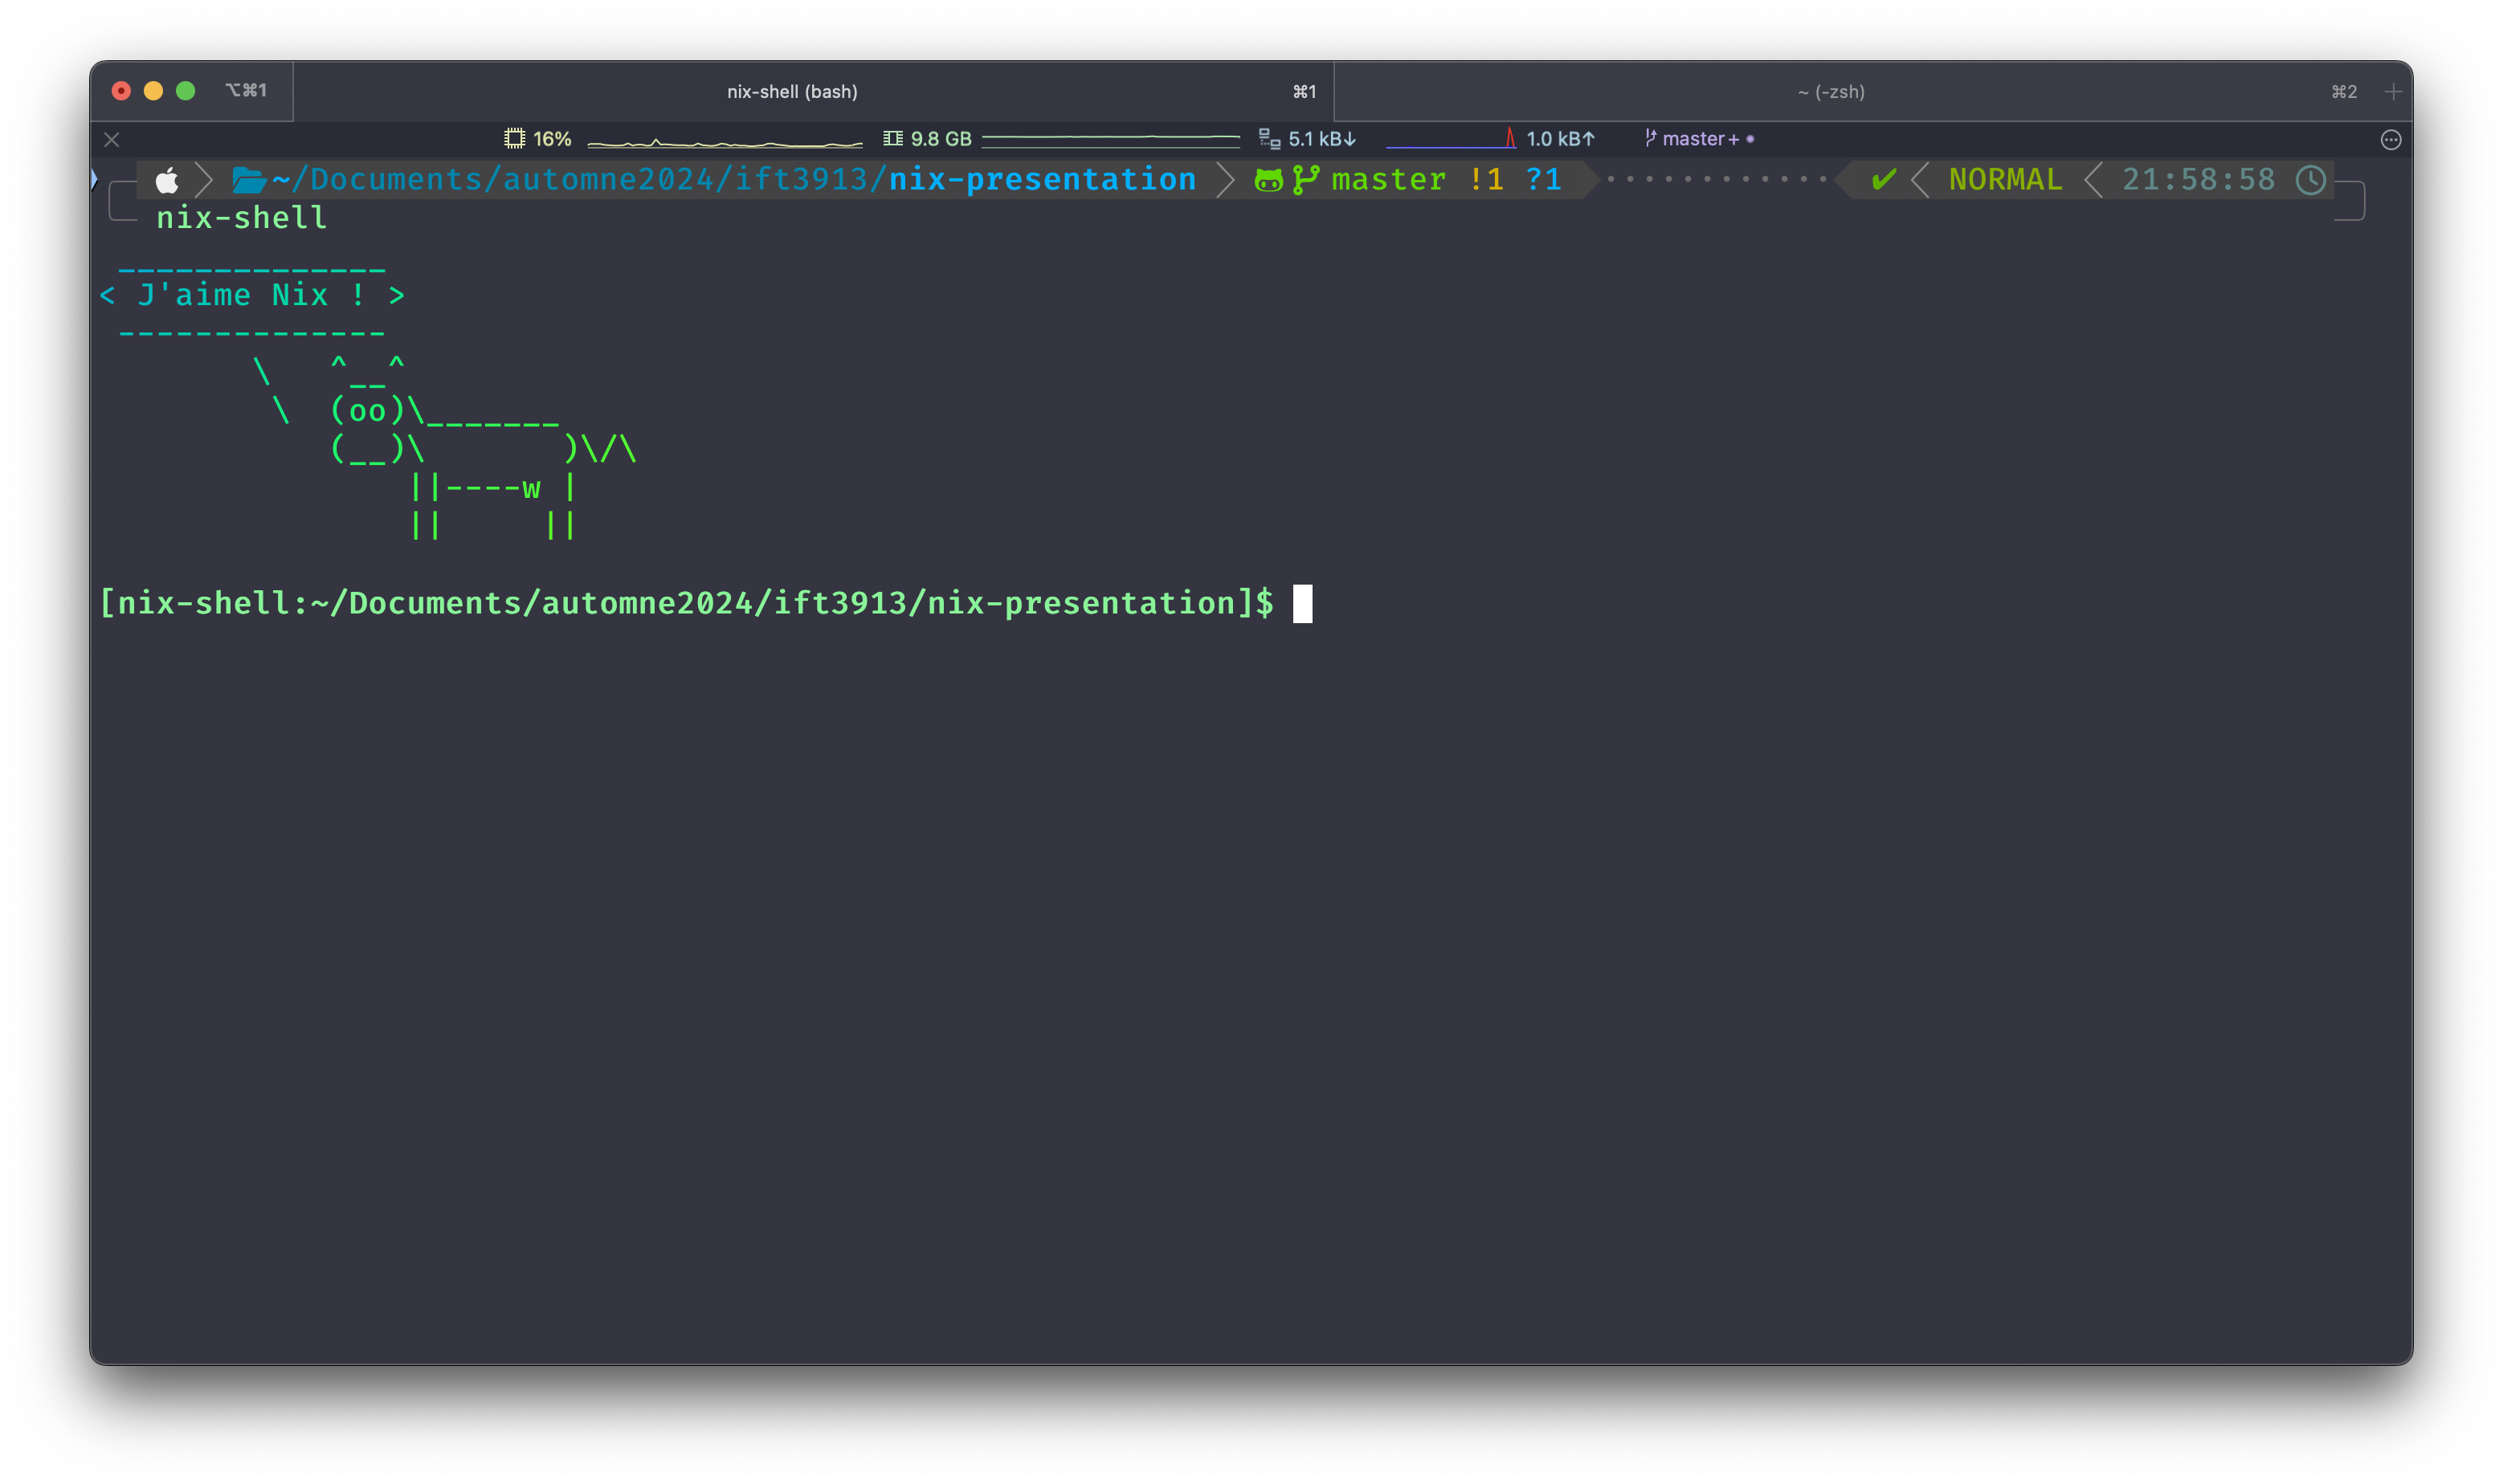
\includegraphics[width=\linewidth]{sg.png}
  \end{center}
\end{frame}




\begin{frame}[fragile]{Installation de Paquets}
	\begin{itemize}
		\item Installation isolée :
	\end{itemize}
	\begin{lstlisting}[language=bash]
$ nix-env -iA nixpkgs.hello
    \end{lstlisting}
	\begin{itemize}
		\item Aucun impact sur les autres paquets
		\item Désinstallation propre
	\end{itemize}
\end{frame}

\section{Point Original}

\begin{frame}{Nix et la Gestion Multi-Utilisateurs}
	\begin{itemize}
		\item Chaque utilisateur peut avoir son propre profil
		\item Partage efficace des ressources communes
		\item Sécurité renforcée
	\end{itemize}
	\footnotetext[4]{\href{https://nixos.org/manual/nix/stable/\#sec-multi-user-installation}{Installation multi-utilisateurs}}
\end{frame}

\section{Réflexion}

\begin{frame}{Avantages et Défis}
    \textbf{Avantages} :
    \begin{itemize}
        \item Environnements cohérents et reproductibles.
        \item Déploiement simplifié pour les équipes de développement.
    \end{itemize}
    \textbf{Défis} :
    \begin{itemize}
        \item Courbe d'apprentissage pour les nouveaux utilisateurs.
        \item Intégration avec les systèmes existants peut être complexe.
        \item Nécessité de comprendre le modèle fonctionnel pour maximiser son potentiel.
    \end{itemize}
    Bien que Nix offre des avantages significatifs, il nécessite un investissement initial en temps d'apprentissage.
\end{frame}
\section{Conclusion}
\begin{frame}{Message Clé}
    \begin{block}{Pourquoi adopter Nix ?}
        \begin{itemize}
            \item \textbf{Contrôle total} sur les environnements, pour éviter les erreurs de version.
            \item \textbf{Flexibilité multi-utilisateurs} et gestion facile des dépendances.
            \item \textbf{Reproductibilité} assurée, pour éviter le fameux "ça
              marche sur ma machine".
        \end{itemize}
    \end{block}
    \begin{center}
        \Large Merci de votre attention ! N'hésitez pas à poser des questions.
    \end{center}
\end{frame}
\begin{frame}{Questions}
	\begin{center}
		\Large Des questions ?
	\end{center}
\end{frame}

\appendix

\section{Sources}

\begin{frame}{Sources}
	\begin{enumerate}
		\item \href{https://nixos.org/}{Site officiel de Nix}
		\item \href{https://nixos.org/manual/nix/stable/}{Manuel de Nix}
		\item \href{https://nixos.org/manual/nixpkgs/stable/}{Guide Nixpkgs}
	\end{enumerate}
\end{frame}

\end{document}
